% SC4024 --- Chapter 6: Volume & Scientific Visualisation (0->100 ground-up)
\chapter{Volume \& Scientific Visualisation}
\label{ch:volume-scientific}
\sloppy

\begin{quote}
\emph{``A CT scan is a stack of shadows; visualisation turns shadows into substance.''} --- From medical volumes to fluid flows, science measures fields, not just tables. This chapter shows how to see them.
\end{quote}

\noindent\fbox{\parbox{\dimexpr\linewidth-2\fboxsep-2\fboxrule}{%
\textbf{From zero: we build here, no prior scientific visualisation needed.} We start from what a scalar or vector field is, then derive isosurfaces, volume rendering, glyphs, and streamlines, with acceleration and code sketches. No prior graphics is assumed.}}
\vspace{0.4em}

\section*{Learning Outcomes}
After this chapter you will be able to:
\begin{enumerate}[label=(L\arabic*)]
    \item distinguish scalar, vector, and tensor fields and their sampling on grids;
    \item extract isosurfaces via marching cubes and choose isovalues;
    \item design transfer functions and explain direct volume rendering by ray casting;
    \item visualise vector fields via glyphs, streamlines, and line integral convolution;
    \item map scientific domains (medical, flow, geospatial) to appropriate methods and optimise via acceleration.
\end{enumerate}

% ============================================================
\section{Fields on Grids}
\label{sec:fields}
\paragraph{Intuition.} Temperature over a room varies at every point---it is a field. A CT scan samples density at voxels (3-D pixels) on a regular grid. A wind simulation samples velocity vectors at grid points. Visualisation must reconstruct the continuous field from these samples and show structure within it.

\paragraph{Formal view.} A \emph{scalar field} $f:\mathbb{R}^3\to\mathbb{R}$ (pressure, density); a \emph{vector field} $\mathbf{v}:\mathbb{R}^3\to\mathbb{R}^3$ (velocity, force); a \emph{tensor field} maps to matrices (stress, diffusion). Data are \emph{sampled} on grids: regular (voxels), rectilinear, structured curvilinear, or unstructured (tetrahedra). Reconstruction uses interpolation (trilinear, higher-order); filtering smooths; gradient $\nabla f$ enables shading.

\begin{definition}[Grid types]\label{def:grids}
\emph{Voxel grid}: regular $n_x\times n_y\times n_z$ with spacing $h$. \emph{Cell}: the cube between 8 neighbours; its value is interpolated. \emph{Scattered}: points with no regular connectivity; triangulation required. Medical CT/MRI and simulation outputs are typically regular grids; geospatial may be terrain + layers.
\end{definition}

\begin{figure}[h]\centering
\begin{tikzpicture}[scale=0.78,every node/.style={font=\scriptsize}]
% volume pipeline
\node[draw,thick,fill=orange!15,rounded corners=4pt,minimum width=2.3cm,minimum height=1.0cm,align=center] (a) at (0,2.0) {Scalar field\\{\tiny $f(x,y,z)$ on grid}};
\node[draw,thick,fill=violet!12,rounded corners=4pt,minimum width=2.3cm,minimum height=1.0cm,align=center] (b) at (3.8,2.0) {Transfer function\\{\tiny value $\to$ colour/opacity}};
\node[draw,thick,fill=blue!14,rounded corners=4pt,minimum width=2.3cm,minimum height=1.0cm,align=center] (c) at (7.6,2.0) {Ray casting\\{\tiny composite along ray}};
\node[draw,thick,fill=green!14,rounded corners=4pt,minimum width=2.3cm,minimum height=1.0cm,align=center] (d) at (11.4,2.0) {Image\\{\tiny pixel colours}};
\draw[->,thick,>=Stealth] (a)--(b) node[midway,above,font=\tiny] {classify};
\draw[->,thick,>=Stealth] (b)--(c) node[midway,above,font=\tiny] {map};
\draw[->,thick,>=Stealth] (c)--(d) node[midway,above,font=\tiny] {accumulate};
% voxel sketch below
\begin{scope}[yshift=-0.8cm]
\draw[thick,fill=blue!8] (0,0) -- (1.2,0.5) -- (1.2,1.7) -- (0,1.2) -- cycle;
\draw[thick,fill=blue!12] (0,1.2) -- (1.2,1.7) -- (2.4,1.7) -- (1.2,1.2) -- cycle;
\draw[thick,fill=blue!6] (1.2,0.5) -- (2.4,0.5) -- (2.4,1.7) -- (1.2,1.7) -- cycle;
\draw[dashed,gray] (0,0) -- (1.2,0.5); \draw[dashed,gray] (0,0) -- (0,1.2);
\fill[red!70] (0.6,0.6) circle (0.07) node[below,font=\tiny] {voxel};
\fill[orange!70] (1.8,1.0) circle (0.07) node[below,font=\tiny] {cell};
\node[font=\tiny,fill=blue!8,rounded corners=2pt] at (3.6,0.8) {trilinear interp. inside cell};
% ray
\draw[->,thick,orange!70!black,>=Stealth] (5.6,0.2) -- (9.0,1.4) node[midway,above,font=\tiny] {ray};
\foreach \x in {6.2,6.7,7.2,7.7,8.2} \fill[orange!60] (\x,0.5+0.22*\x-1.0) circle (0.05);
\node[font=\tiny,fill=orange!10,rounded corners=2pt] at (7.3,0.1) {samples along ray};
% transfer curve
\begin{scope}[xshift=9.8cm]
\draw[->,thick] (0,0) -- (2.2,0) node[below,font=\tiny] {value};
\draw[->,thick] (0,0) -- (0,1.4) node[left,font=\tiny] {opac.};
\draw[thick,violet!60!black,smooth] plot coordinates {(0,0.1) (0.8,0.15) (1.1,0.9) (1.6,1.0) (2.0,0.95)};
\node[font=\tiny,fill=violet!8,rounded corners=2pt] at (1.1,-0.35) {transfer function};
\end{scope}
\end{scope}
\node[font=\tiny,draw=gray!40,fill=yellow!8,rounded corners=2pt,inner sep=3pt] at (5.8,-1.35) {\textcolor{orange!70!black}{$\blacksquare$ field} \quad \textcolor{violet!60!black}{$\blacksquare$ transfer} \quad \textcolor{blue!60!black}{$\blacksquare$ ray} \quad \textcolor{green!50!black}{$\blacksquare$ image}};
\end{tikzpicture}
\caption{Volume rendering pipeline (top): field $\to$ transfer function $\to$ ray casting $\to$ image. Bottom: voxel/cell with trilinear interpolation, sampling along a ray, and an opacity transfer function.}
\label{fig:volume-pipeline}
\end{figure}

% ============================================================
\section{Scalar Fields: Isosurfaces and Volume Rendering}
\label{sec:scalar}
\paragraph{Intuition.} An isosurface is the 3-D equivalent of a contour line: the set $\{x\mid f(x)=k\}$ for chosen isovalue $k$. Pick $k$ to be skin vs bone in CT and the surface appears. Volume rendering instead shows the whole volume with translucency: bone opaque, flesh semi-transparent, air invisible---controlled by the transfer function.

\begin{definition}[Marching cubes and ray casting]\label{def:marching}
\emph{Marching cubes}: for each cube of 8 voxels, classify each vertex as inside ($f>k$) or outside; use a 256-case table (15 unique) to emit triangles interpolating edge intersections. \emph{Direct volume rendering}: for each pixel cast a ray, sample $f$ at steps, map via transfer function to colour/opacity $(c,\alpha)$, composite front-to-back: $C=\sum c_i\alpha_i\prod_{j<i}(1-\alpha_j)$.
\end{definition}

\begin{figure}[h]\centering
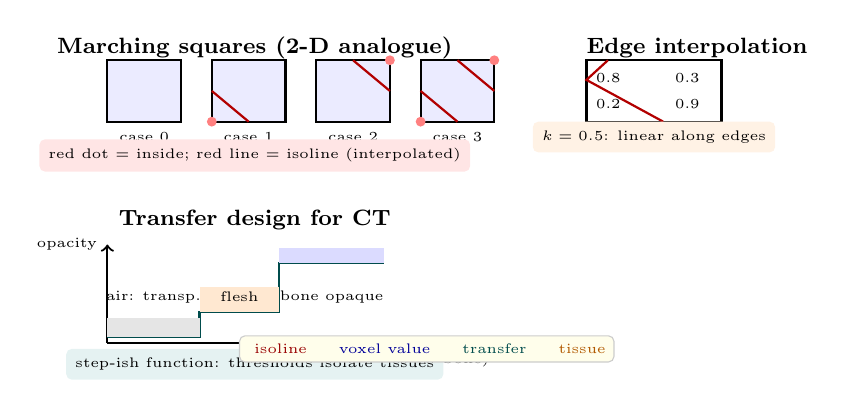
\begin{tikzpicture}[scale=0.78,every node/.style={font=\scriptsize}]
% 2D marching squares cases
\node[font=\footnotesize\bfseries] at (2.4,4.2) {Marching squares (2-D analogue)};
\foreach \case/\x in {0/0,1/1.7,2/3.4,3/5.1} {
  \draw[thick,fill=blue!8] (\x,3.0) rectangle +(1.2,1.0);
  \ifnum\case=1 \fill[red!50] (\x,3.0) circle (0.08); \draw[thick,red!70!black] (\x+0.6,3.0) -- (\x,3.5);
  \fi \ifnum\case=2 \fill[red!50] (\x+1.2,4.0) circle (0.08); \draw[thick,red!70!black] (\x+0.6,4.0) -- (\x+1.2,3.5);
  \fi \ifnum\case=3 \fill[red!50] (\x,3.0) circle (0.08); \fill[red!50] (\x+1.2,4.0) circle (0.08); \draw[thick,red!70!black] (\x+0.6,3.0) -- (\x,3.5); \draw[thick,red!70!black] (\x+0.6,4.0) -- (\x+1.2,3.5); \fi
  \node[font=\tiny] at (\x+0.6,2.75) {case \case};
}
\node[font=\tiny,fill=red!10,rounded corners=2pt] at (2.4,2.45) {red dot = inside; red line = isoline (interpolated)};
% interpolation detail
\begin{scope}[xshift=7.8cm]
\node[font=\footnotesize\bfseries] at (1.8,4.2) {Edge interpolation};
\draw[thick] (0,3.0) rectangle (2.2,4.0);
\node[font=\tiny] at (0,3.05) [anchor=south west] {0.2};
\node[font=\tiny] at (2.0,3.05) [anchor=south east] {0.9};
\node[font=\tiny] at (0,3.95) [anchor=north west] {0.8};
\node[font=\tiny] at (2.0,3.95) [anchor=north east] {0.3};
\draw[thick,red!70!black] (1.25,3.0) -- (0,3.68) -- (0.35,4.0);
\node[font=\tiny,fill=orange!10,rounded corners=2pt] at (1.1,2.75) {$k=0.5$: linear along edges};
\end{scope}
% transfer function design
\begin{scope}[yshift=-0.6cm]
\node[font=\footnotesize\bfseries] at (2.4,2.0) {Transfer design for CT};
\draw[->,thick] (0,0) -- (4.8,0) node[below,font=\tiny] {density (air $\to$ bone)};
\draw[->,thick] (0,0) -- (0,1.6) node[left,font=\tiny] {opacity};
\draw[thick,teal!60!black] (0,0.1) -- (1.5,0.1) -- (1.5,0.5) -- (2.8,0.5) -- (2.8,1.3) -- (4.5,1.3);
\fill[gray!20] (0,0.1) rectangle (1.5,0.4); \node[font=\tiny] at (0.75,0.75) {air: transp.};
\fill[orange!18] (1.5,0.5) rectangle (2.8,0.9); \node[font=\tiny] at (2.15,0.75) {flesh};
\fill[blue!14] (2.8,1.3) rectangle (4.5,1.55); \node[font=\tiny] at (3.65,0.75) {bone opaque};
\node[font=\tiny,fill=teal!10,rounded corners=2pt] at (2.4,-0.35) {step-ish function: thresholds isolate tissues};
\end{scope}
\node[font=\tiny,draw=gray!40,fill=yellow!8,rounded corners=2pt,inner sep=3pt] at (5.2,-0.70) {\textcolor{red!60!black}{$\blacksquare$ isoline} \quad \textcolor{blue!60!black}{$\blacksquare$ voxel value} \quad \textcolor{teal!60!black}{$\blacksquare$ transfer} \quad \textcolor{orange!70!black}{$\blacksquare$ tissue}};
\end{tikzpicture}
\caption{Scalar fields: 2-D marching squares cases (top left), edge interpolation for isovalue $k$ (top right), and a CT transfer function mapping density to opacity (bottom). Marching cubes extends this to 8-vertex cubes with triangles.}
\label{fig:marching}
\end{figure}

Transfer design is the craft: too narrow a window and you hide anatomy; too wide and everything is translucent fog. Histogram of voxel values plus gradient magnitude guides placement of opacity ramps at material boundaries.

% ============================================================
\section{Vector and Tensor Fields}
\label{sec:vector}
\paragraph{Intuition.} Wind at each point has direction and speed---an arrow. But thousands of arrows occlude; streamlines that follow the wind tell the story more cleanly, and a texture smeared along the flow (LIC) shows it everywhere at once.

\begin{definition}[Glyphs, streamlines, LIC]\label{def:vector-vis}
\emph{Glyph}: an icon (arrow, ellipsoid) at sampled points encoding vector magnitude/direction (and tensor shape). \emph{Streamline}: curve $x(t)$ with $dx/dt=\mathbf{v}(x)$ from a seed, integrated via Euler or Runge--Kutta; streamsurface for dense seeds; streamsurface/pillars for 3-D. \emph{Line integral convolution (LIC)}: convolve noise texture along streamlines to produce streaks coherent with flow, revealing topology without seeding.
\end{definition}

\begin{figure}[h]\centering
\begin{tikzpicture}[scale=0.75,every node/.style={font=\scriptsize}]
% glyphs
\begin{scope}
\node[font=\footnotesize\bfseries] at (1.6,3.4) {Glyphs (sampled)};
\foreach \x in {0.4,1.2,2.0} \foreach \y in {0.6,1.4,2.2} {
  \pgfmathsetmacro{\dx}{0.3*cos(20+30*\x+15*\y)} \pgfmathsetmacro{\dy}{0.3*sin(20+30*\x+15*\y)}
  \draw[->,thick,>=Stealth,green!60!black] (\x,\y) -- ++(\dx,\dy);
}
\node[font=\tiny,fill=green!10,rounded corners=2pt] at (1.6,0.2) {arrow = direction+speed};
\end{scope}
% streamlines
\begin{scope}[xshift=4.2cm]
\node[font=\footnotesize\bfseries] at (1.8,3.4) {Streamlines (integrated)};
\draw[->,thick,blue!60!black,smooth] plot coordinates {(0.2,0.6) (0.9,1.0) (1.6,1.6) (2.2,2.2) (2.8,2.4)};
\draw[->,thick,blue!60!black,smooth] plot coordinates {(0.4,2.4) (1.1,2.0) (1.9,1.4) (2.6,0.9)};
\draw[->,thick,blue!60!black,smooth] plot coordinates {(0.2,1.4) (0.8,1.5) (1.5,1.7) (2.2,1.8)};
\fill[red!60] (0.2,0.6) circle (0.06); \fill[red!60] (0.4,2.4) circle (0.06); \fill[red!60] (0.2,1.4) circle (0.06);
\node[font=\tiny,fill=red!10,rounded corners=2pt] at (1.8,0.2) {red = seeds; curves follow $\mathbf{v}$};
\end{scope}
% LIC texture
\begin{scope}[xshift=8.4cm]
\node[font=\footnotesize\bfseries] at (1.8,3.4) {LIC (dense texture)};
\fill[gray!8] (0,0.4) rectangle (3.6,2.8);
\foreach \y in {0.6,0.9,...,2.6} {
  \draw[gray!40,thin,smooth] plot coordinates {(0.2,\y) (0.9,\y+0.1) (1.6,\y+0.15) (2.3,\y+0.1) (3.0,\y) (3.4,\y-0.05)};
}
\foreach \y in {0.75,1.05,...,2.45} {
  \draw[gray!55,thin,smooth] plot coordinates {(0.2,\y) (1.0,\y+0.08) (1.8,\y+0.12) (2.6,\y+0.05)};
}
\node[font=\tiny,fill=gray!12,rounded corners=2pt] at (1.8,0.2) {streaks coherent with flow};
\end{scope}
% tensor ellipsoids
\begin{scope}[xshift=12.4cm]
\node[font=\footnotesize\bfseries] at (1.2,3.4) {Tensor ellipsoids};
\draw[fill=violet!14,draw=violet!60!black] (0.6,2.0) ellipse (0.45 and 0.22);
\draw[fill=violet!10,draw=violet!60!black] (0.6,1.2) ellipse (0.30 and 0.30);
\draw[fill=orange!14,draw=orange!60!black] (1.8,1.6) ellipse (0.40 and 0.18);
\node[font=\tiny,fill=violet!8,rounded corners=2pt] at (1.2,0.2) {axes = eigenvectors};
\end{scope}
\node[font=\tiny,draw=gray!40,fill=yellow!8,rounded corners=2pt,inner sep=3pt] at (6.8,-0.25) {\textcolor{green!50!black}{$\blacksquare$ glyph} \quad \textcolor{blue!60!black}{$\blacksquare$ streamline} \quad \textcolor{gray!60!black}{$\blacksquare$ LIC} \quad \textcolor{violet!60!black}{$\blacksquare$ tensor}};
\end{tikzpicture}
\caption{Vector field views: glyphs at samples (left), streamlines from seeds (centre), LIC dense texture (centre-right), and tensor ellipsoids (right). Density and occlusion trade off across methods.}
\label{fig:vector}
\end{figure}

Tensors (diffusion MRI, stress) add shape: an ellipsoid's axes are eigenvectors, lengths are eigenvalues; isotropy vs anisotropy maps to fractional anisotropy colour (red $x$, green $y$, blue $z$).

% ============================================================
\section{Domains, Projections, and Acceleration}
Domains: \emph{medical} (CT/MRI iso + volume), \emph{flow} (CFD streamlines/LIC), \emph{geospatial} (terrain + fields + map projections: Mercator, equal-area), \emph{time-varying} (animation or space-time cube). Acceleration: \emph{octrees/bricks} skip empty space, \emph{early ray termination} stops when opacity saturates, \emph{level-of-detail} and \emph{GPU ray casting} exploit parallelism.

\begin{lstlisting}[language=Python, caption={Marching cubes isosurface with scikit-image.}, label={lst:marching-code}]
import numpy as np
from skimage import measure
import matplotlib.pyplot as plt
from mpl_toolkits.mplot3d.art3d import Poly3DCollection

# Synthetic scalar field: two blobs
x,y,z = np.ogrid[-3:3:40j, -3:3:40j, -3:3:40j]
field = np.exp(-((x-1)**2+y**2+z**2)) + 0.7*np.exp(-((x+1)**2+y**2+z**2))
verts, faces, _, _ = measure.marching_cubes(field, level=0.5)  # isovalue
fig = plt.figure(); ax = fig.add_subplot(111, projection="3d")
mesh = Poly3DCollection(verts[faces], alpha=0.7, edgecolor="none", facecolor="steelblue")
ax.add_collection3d(mesh); ax.set_xlim(0,40); ax.set_ylim(0,40); ax.set_zlim(0,40)
plt.title("Isosurface at k=0.5"); plt.savefig("isosurface.pdf")
\end{lstlisting}

\begin{lstlisting}[language=Python, caption={Volume ray-marching sketch (front-to-back compositing).}, label={lst:raymarch}]
import numpy as np

def ray_march(field, ray_origin, ray_dir, transfer, steps=128, dt=0.05):
    """field: 3-D array; transfer: value -> (r,g,b,alpha); returns pixel colour."""
    pos = np.array(ray_origin, float); colour = np.zeros(3); alpha_acc = 0.0
    for _ in range(steps):
        v = trilinear(field, pos)          # interpolate
        r,g,b,a = transfer(v)
        # front-to-back compositing
        colour += (1-alpha_acc) * a * np.array([r,g,b])
        alpha_acc += (1-alpha_acc) * a
        if alpha_acc >= 0.99: break        # early termination
        pos += dt * np.array(ray_dir)
    return colour

def trilinear(vol, p):
    # placeholder: clamp and trilinearly interpolate vol at continuous p
    return float(np.clip(vol[int(p[0])%vol.shape[0], int(p[1])%vol.shape[1], int(p[2])%vol.shape[2]], 0, 1))

def transfer_ct(v):
    # toy CT: air transparent, flesh pink semi, bone white opaque
    if v < 0.3: return (0,0,0,0.0)
    elif v < 0.6: return (0.9,0.6,0.6,0.2)
    else: return (1,1,1,0.9)
\end{lstlisting}

% ============================================================
\section{Chapter Notes}
Lorensen and Cline (1987) introduced marching cubes; Levoy (1988) and Drebin et al.\ formulated volume rendering; Cabral and Leedom (1993) gave LIC; map projections date to Mercator (1569) with modern equal-area alternatives; acceleration via octrees and GPU ray casting surveyed by Engel et al. The next chapter asks whether these pictures actually help humans think.

% ============================================================
\section{Exercises}
\label{sec:ch06-exercises}
\begin{enumerate}[label=E6.\arabic*, leftmargin=*, itemsep=0.8em]
    \item \textbf{Isocontour by hand.} On a $2\times2$ grid with values $0.2,0.9$ (top) and $0.8,0.3$ (bottom), extract the $k=0.5$ isoline via marching squares. List edge intersections by linear interpolation and draw the line segments.
    \item \textbf{Transfer design.} Given a CT histogram with peaks at $0.1$ (air), $0.5$ (soft tissue), $0.85$ (bone), sketch an opacity transfer function that isolates each tissue. Explain the effect of widening the bone window.
    \item \textbf{Streamline integration.} For $\mathbf{v}(x,y)=(-y,x)$ (rotation), trace a streamline from $(1,0)$ using Euler with $dt=0.2$ for 5 steps and compare to the true circle. Why does Euler spiral outward?
    \item \textbf{LIC vs glyphs.} For a turbulent field with 10k vectors, argue when LIC beats glyphs and when glyphs beat LIC, considering occlusion, seed dependence, and ability to read magnitude.
    \item \textbf{Octree culling.} A $512^3$ volume is 70\% empty (value $<$ threshold). Estimate memory and ray-step savings from an octree that culls empty bricks of $32^3$. When does early ray termination give additional gain?
\end{enumerate}
% End of Chapter 6
